\section{Experimental Evaluation}
\label{sec:xps}



\begin{table}[]
    \centering
    \definecolor{darkgreen}{HTML}{005701}
    \newcommand{\withmod}{\checkmark}
    \newcommand{\withoutmod}{$\times$}
    \newcommand{\firstcell}[1]{#1 & }
    \newcommand{\onediffcell}[2]{#1 & \textcolor{darkgreen}{\small (+#2)}}
    \resizebox{\linewidth}{!}{
    \begin{tabular}{c|c@{~~}c@{~~}c@{~~}c@{~~}c|r@{}rr@{}rr@{}rr@{}r}
\toprule
 & \multicolumn{5}{c|}{aux. modalities} & \multicolumn{2}{c}{focal} & \multicolumn{2}{c}{depth} & \multicolumn{4}{c}{rel. pose} \\
 & K1 & K2 & D1 & D2 & RT & \multicolumn{2}{c}{acc@1.015} & \multicolumn{2}{c}{$\tau$@1.03} & \multicolumn{2}{c}{RRA@2$^\circ$} & \multicolumn{2}{c}{RTA@2$^\circ$} \\
\midrule
DUSt3R & \withoutmod & \withoutmod & \withoutmod & \withoutmod & \withoutmod & \firstcell{36.6} & \firstcell{77.6} & \firstcell{69.2} & \firstcell{49.7} \\
\midrule
\multirow{12}{*}{\textbf{\ours{}}} & \withoutmod & \withoutmod & \withoutmod & \withoutmod & \withoutmod & \firstcell{39.4} & \firstcell{79.4} & \firstcell{71.9} & \firstcell{53.8} \\
 & \withmod & \withoutmod & \withoutmod & \withoutmod & \withoutmod & \onediffcell{75.4}{36.0} & \onediffcell{80.6}{1.2} & \onediffcell{77.1}{5.3} & \onediffcell{62.8}{8.9} \\
 & \withoutmod & \withmod & \withoutmod & \withoutmod & \withoutmod & \onediffcell{67.3}{27.9} & \onediffcell{80.3}{0.9} & \onediffcell{74.5}{2.6} & \onediffcell{59.1}{5.2} \\
 & \withmod & \withmod & \withoutmod & \withoutmod & \withoutmod & \onediffcell{98.0}{58.6} & \onediffcell{81.4}{2.0} & \onediffcell{80.3}{8.5} & \onediffcell{74.2}{20.3} \\
 & \withoutmod & \withoutmod & \withmod & \withoutmod & \withoutmod & \onediffcell{48.9}{9.5} & \onediffcell{89.1}{9.7} & \onediffcell{82.5}{10.6} & \onediffcell{64.9}{11.0} \\
 & \withoutmod & \withoutmod & \withoutmod & \withmod & \withoutmod & \onediffcell{49.5}{10.1} & \onediffcell{91.0}{11.7} & \onediffcell{83.4}{11.5} & \onediffcell{64.8}{10.9} \\
 & \withoutmod & \withoutmod & \withmod & \withmod & \withoutmod & \onediffcell{58.2}{18.9} & \onediffcell{\textbf{95.4}}{\textbf{16.0}} & \onediffcell{89.6}{17.7} & \onediffcell{77.6}{23.8} \\
 & \withoutmod & \withoutmod & \withoutmod & \withoutmod & \withmod & \onediffcell{48.6}{9.2} & \onediffcell{81.6}{2.2} & \onediffcell{92.3}{20.5} & \onediffcell{77.0}{23.1} \\
 & \withmod & \withmod & \withmod & \withmod & \withoutmod & \onediffcell{99.2}{59.8} & \onediffcell{\textbf{95.4}}{\textbf{16.0}} & \onediffcell{95.7}{23.9} & \onediffcell{94.3}{40.5} \\
 & \withmod & \withmod & \withoutmod & \withoutmod & \withmod & \onediffcell{98.1}{58.7} & \onediffcell{82.9}{3.6} & \onediffcell{95.1}{23.2} & \onediffcell{87.3}{33.5} \\
 & \withoutmod & \withoutmod & \withmod & \withmod & \withmod & \onediffcell{68.6}{29.2} & \onediffcell{\textbf{95.4}}{\textbf{16.0}} & \onediffcell{98.1}{26.2} & \onediffcell{91.3}{37.5} \\
 & \withmod & \withmod & \withmod & \withmod & \withmod & \onediffcell{\textbf{99.3}}{\textbf{59.9}} & \onediffcell{\textbf{95.4}}{\textbf{16.0}} & \onediffcell{\textbf{99.0}}{\textbf{27.2}} & \onediffcell{\textbf{98.1}}{\textbf{44.3}} \\
\bottomrule





    \end{tabular}
    }
    \vspace{-0.3cm}
    \caption{\textbf{Impact of guiding at test time} for models trained at $224{\times}224$ resolution. We report performances on Habitat for DUSt3R, which cannot handle auxiliary modalities, and our single model with different sets of modalities; we show in green the absolute improvement \wrt the results without auxiliary modality.
    }
    \vspace{-0.4cm}
    \label{tab:modality_study}
\end{table}




We first study the impact of auxiliary information guidance  (\cref{sec:xp_guiding}). 
We then experiment across many 3D vision tasks (\cref{sec:xp_mvd,sec:xp_mvds,sec:xp_mvstereo}) without retraining, \ie mostly zero-shot settings. We finally present some ablations in \cref{sec:ablations}.

\myparagraph{\duster{} baseline.}
We point out that our overall training data, protocols and architecture are exactly the same as \duster{}, except for the additional head that predict $\X{2}{2}$ (+0.1\% parameters) and for the modules used for injecting the auxiliary information (+4\% parameters for the \inject{1} variant that we use unless stated otherwise). 


\myparagraph{Metrics.}
When evaluating focal lengths, we report the accuracy for a tight relative error threshold of 1.5\%.
For evaluating depthmap, we report the Absolute Relative Error (rel) and the Inlier Ratio ($\tau$) at a threshold of 3\%.
When evaluating poses, we opt for scale-invariant metrics and measure the relative rotation and translation accuracies (RRA and RTA resp.) of the relative pose at task-specific thresholds, and the mean Average Accuracy (mAA), defined as the area under the curve accuracy of the angular differences at min(RRA, RTA). %




\subsection{Guiding the output prediction}
\label{sec:xp_guiding}

\myparagraph{Impact of guidance.}
We first study the impact of providing different subsets of auxiliary information in terms of downstream 3D vision performance.
Namely, we report accuracies in \cref{tab:modality_study} for focal, depth, and rotation prediction on the Habitat validation dataset. %
In the supplementary material, we also provide results on the Infinigen dataset~\cite{Raistrick2023Infinigen}, which is not included in our training set, and observe similar outcomes.
We first note that in the absence of modalities, \ours{} performs slightly better than a \duster{} baseline, even though \ours{} is trained with just RGB images during a fraction of its training.
This shows that \ours{} does not lose its native strength for unconstrained regression despite having gained more capabilities.

Interestingly, we observe in \cref{tab:modality_study} the impact of each modality for each prediction task, and the synergetic effects of interacting modalities.
For instance, the model performs better for focal length estimation with depthmaps and/or relative pose, and \ours{}'s depth prediction improves with intrinsics and/or relative pose.
Moreover, relative pose prediction becomes more accurate with intrinsics and/or depthmap.
Overall, the model's performance consistently improves when provided with additional camera or scene priors, demonstrating the effectiveness of \ours in handling any combination of priors in a unified fashion.
We are not aware of any other approach that can seamlessly integrate all these priors in a learning-based method.


\begin{figure}
    \centering
    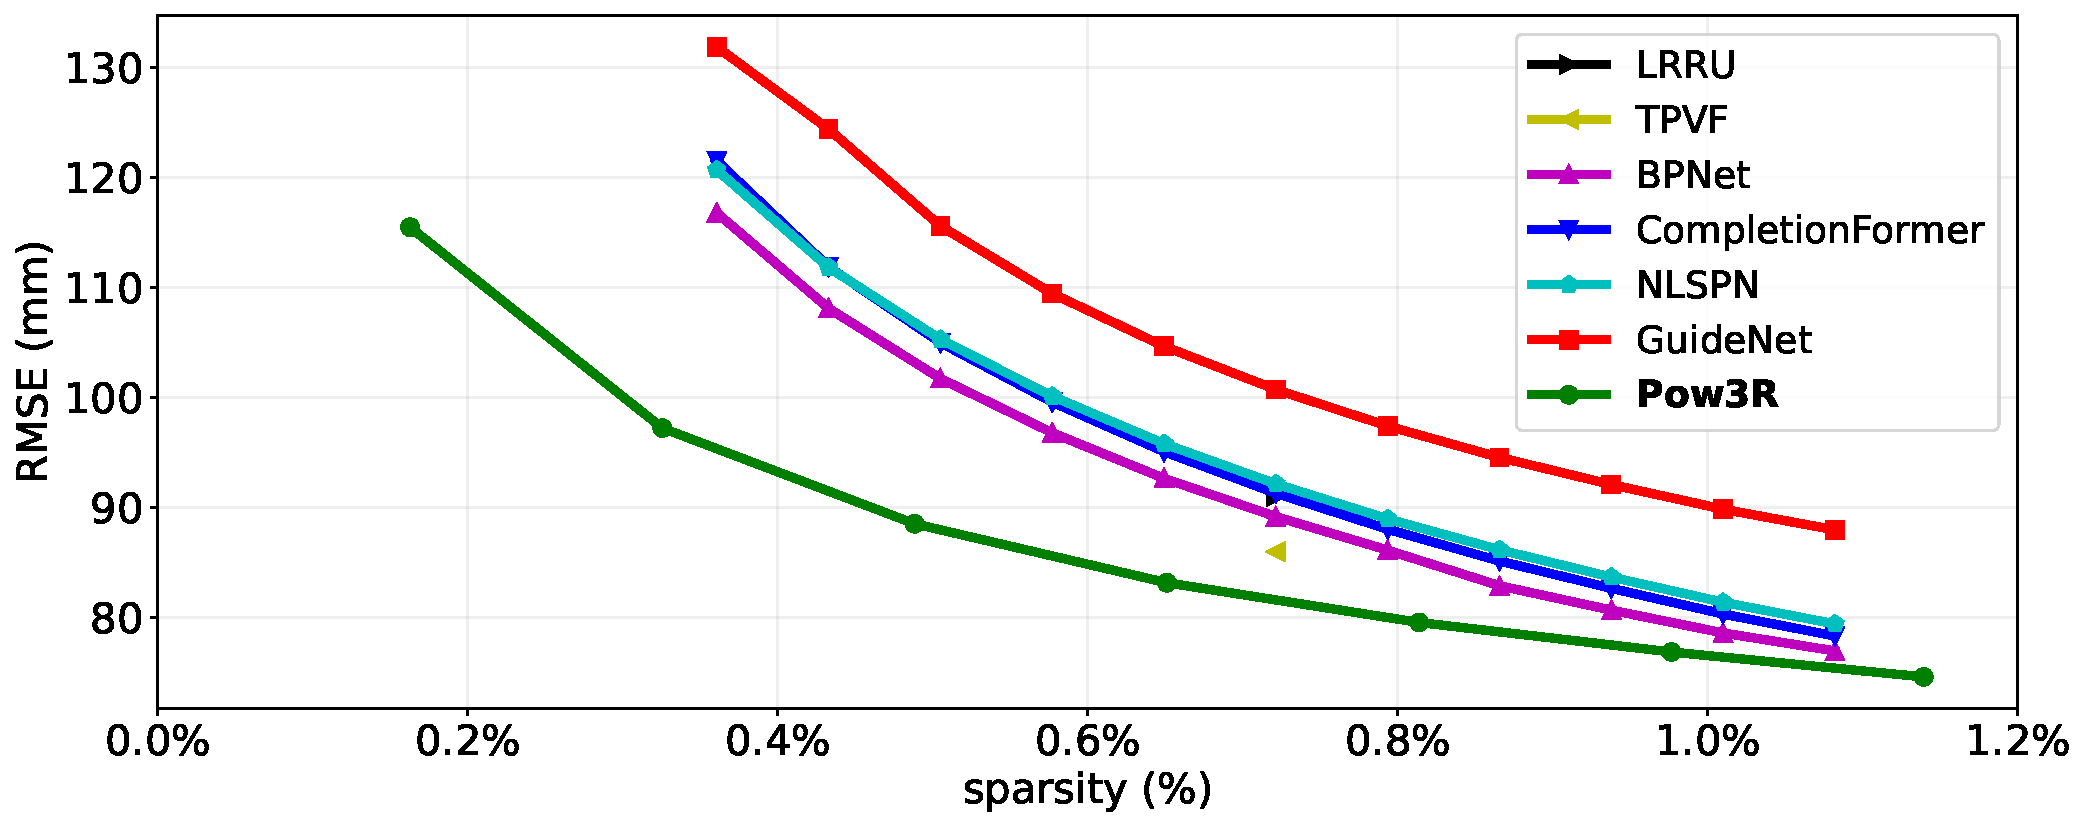
\includegraphics[width=\linewidth]{figures/depthcompletion/depth_completion_nyu_sparsity.pdf} \\[-0.4cm]
    \caption{\textbf{Depth completion performance} on NYUd for various input depth sparsity. 
    }
    \vspace{-0.2cm}
    \label{fig:depthcompletion_nyu}
\end{figure}

\myparagraph{Depth completion.}
We also evaluate \ours{} on the depth completion task given RGB images with sparse depthmaps.
We vary the sparsity (the ratio of pixels with known depth) %
and demonstrate its impact on the NYUv2 dataset~\cite{SilbermanHKF12} in Figure~\ref{fig:depthcompletion_nyu}.
Although \ours{} is not trained on the NYUv2 dataset, it still achieves state-of-the-art results for sparse depth completion.
Our analysis indicates that the true performance of \ours{} on NYUv2  is likely underestimated due to numerous errors in the ground-truth depth annotations; further details are available in the supplementary material. %
On the KITTI~\cite{geiger2013vision} dataset, we obtain a mean absolute error below 30cm, which is competitive with the state of the art, 
considering that KITTI is not included in the training set.



\myparagraph{High-Resolution processing.}
With the possibility of specifying camera intrinsics, new capabilities arise.
Namely, \ours{} can perform high-resolution pointmap regression with a simple sliding-window approach.
We process fixed-resolution crops of the original images under the guidance of both (i) the crop information, provided in term of camera intrinsics, and (ii) a second image, itself possibly downscaled or cropped as well.
More details are provided in \cref{sec:applications} and \cref{fig:native_ex}.
When applied, results significantly improve compared to processing the images at 512-pixel resolution, as shown in \cref{tab:native}.
We also compare with a naive baseline where we simply feed high-resolution images directly to \ours{}, but it dramatically fails.

\begin{table}[]
    \centering
    \resizebox{\linewidth}{!}{
    \begin{tabular}{lc@{~}cc|cccccc}
    \toprule 
     & \multicolumn{2}{c}{\small{aux. mod.}} & High- & \multicolumn{2}{c}{KITTI} & & \multicolumn{2}{c}{T\&T} & Time \\
    \cmidrule{5-6} \cmidrule{8-9} 
     & Ks & RT & Res. & rel$\downarrow$ & $\tau\uparrow$ &  & rel$\downarrow$ & $\tau\uparrow$ & (sec)$\downarrow$\\
    \midrule
    \duster{}512 & $\times$ & $\times$ & $\times$ & 5.4 & 49.5 &  & 3.3 & 75.1 & 0.13\\
    \midrule
    \ours{}512 & $\checkmark$ & $\checkmark$ & $\times$ & 5.3 & 48.7 &  & 3.2 & 78.2 & 0.13\\
    \ours{}512 & $\checkmark$ & $\checkmark$ & (n) & 7.5  & 34.4 &  & 3.9 & 68.0 & 0.48\\
    \ours{}512 & $\checkmark$ & $\checkmark$ & $\checkmark$ & \textbf{4.6} & \textbf{53.5} &  & \textbf{2.5} & \textbf{82.3} & 0.40\\
    \bottomrule
    \end{tabular}} \vspace{-0.3cm}
    \caption{\textbf{Multi-view depth estimation results in high-resolution}
        using a sliding-window scheme and providing the crop intrinsics to \ours{}. 
        (n): naively inputting high-resolution images without downsampling to \ours{}.
        }
    \vspace{-0.4cm}
    \label{tab:native}
\end{table}



\myparagraph{Camera controllability.}
We study how \emph{controllable} are the regression outputs on 10K Habitat test pairs given arbitrary camera parameters.
For each test pair with ground-truth focal $f$ and relative pose $P_{12}$, we purposefully input a \emph{wrong} focal (resp. relative pose) and measure the output focal $\hat{f}$ (resp. pose $\hat{P}_{12}$) as predicted from the raw pointmaps.
Results are presented in \cref{fig:controlability} in terms of focal ratio $\nicefrac{\hat{f}}{f}$ and angle $d_{\text{geodesic}}(P_{12}, \hat{P}_{12})$.
Interestingly, the model accepts to follow the guidance whenever it is close to the ground truth value (\ie staying close to the identity transformation) %
but then refuses to follow it when it gets too different, showing that the model is able to somehow `judge' of the guidance's worth.
In all cases, the output confidence clearly correlates with the agreement between the guidance and the ground truth.
Overall, the model is thus not taking the auxiliary information at face value, and instead combines it with the other modalities (\eg RGB) it in a more subtle and informed way than what could be achieved with handcrafted methods.
This suggests that \ours{} would be robust to noise in the auxiliary information.

\begin{figure}
    \centering
    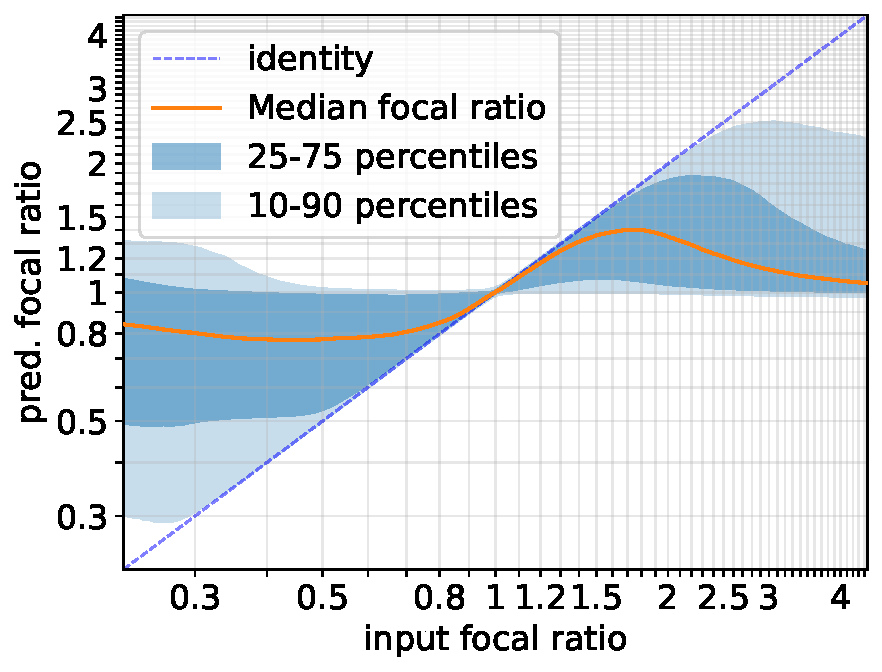
\includegraphics[width=0.49\linewidth]{figures/controllability/fakefocal_plot_K1.pdf} 
    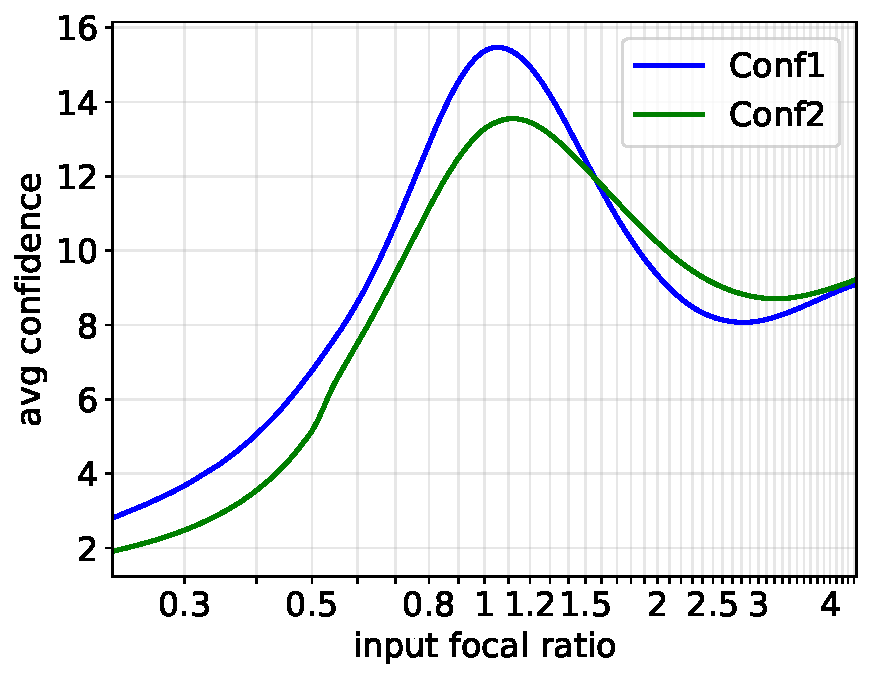
\includegraphics[width=0.49\linewidth]{figures/controllability/fakefocal_plot_conf.pdf} 
    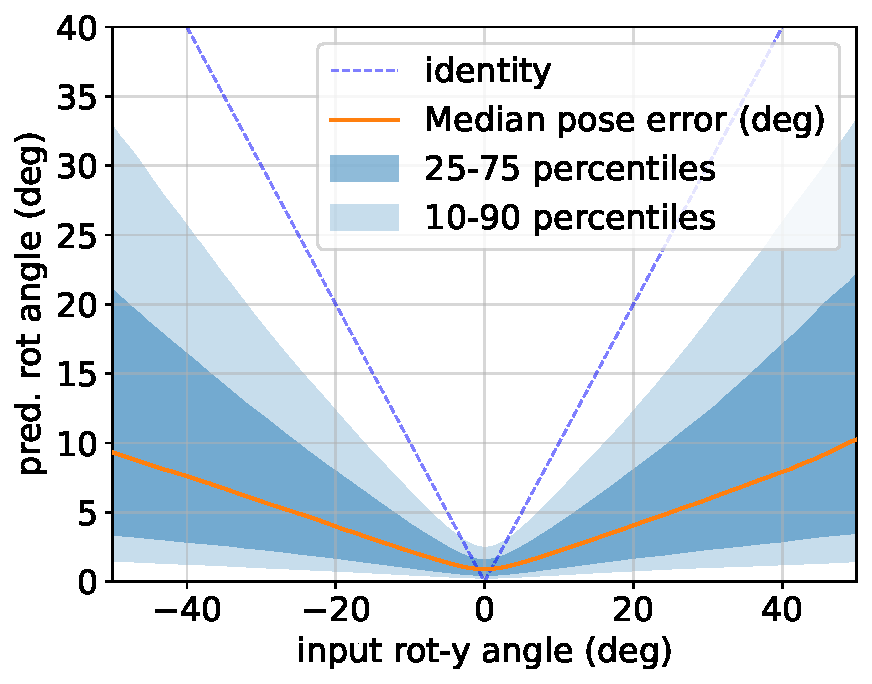
\includegraphics[width=0.49\linewidth]{figures/controllability/fakerelpose_plot.pdf}
    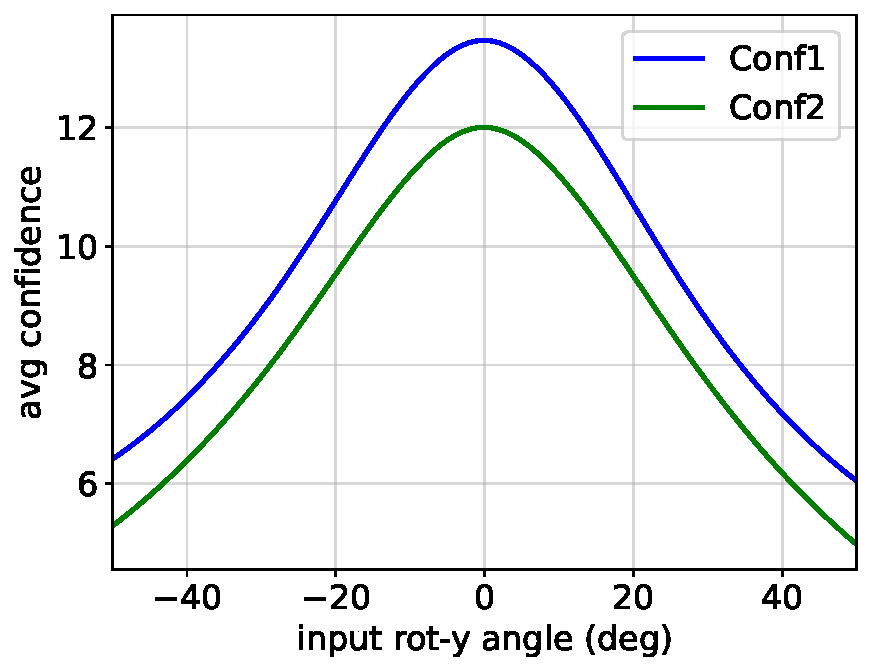
\includegraphics[width=0.49\linewidth]{figures/controllability/fakerelpose_plot_conf.pdf}
    \\[-0.35cm]
    \caption{\textbf{Controllability study}.
        We study how the model reacts when presented with false focal (top) and false relative pose (bottom). We plot the input \emph{vs.} predicted camera parameters in the left column and the average confidence in the right column. Interestingly, the model seems to not take the input information at face value and instead makes an informed decision whether to use it or not, in which latter case the confidence becomes low.
        } 
    \label{fig:controlability}
    \vspace{-0.25cm}
\end{figure}


\subsection{Multi-View Depth Estimation}
\label{sec:xp_mvd}

Following RobustMVD~\cite{schroppel2022benchmark}, performances are measured on the KITTI~\cite{geiger2013vision}, ScanNet~\cite{dai2017scannet}, ETH3D~\cite{schops2017multi}, DTU~\cite{aanaes2016large}, and Tanks and Temples~\cite{knapitsch2017tanks} datasets. %
We report in \cref{tab:mvd} the Absolute Relative Error (rel) and Inlier Ratio ($\tau$) for each dataset when using (1) images alone, (2) images with relative poses, (3) images with camera intrinsics, and (4) images with both 
 modalities, and provide results for more state-of-the-art methods in the supplementary material. %

\myparagraph{Results}.
\ours{} again performs roughly on par with \duster{} in the absence of auxiliary information (\eg 3.73 average error across all datasets for \duster{}-512 \vs 3.64 for \ours{}-512). 
However, it is clear that providing auxiliary information consistently improves the depth estimates. %
In fact, \ours{}-512 with both pose and intrinsics achieves state-of-the-art performance on the ETH3D, DTU, and Tanks and Temples datasets, as well as on average across datasets.
Interestingly, intrinsics tend to improve performance more than the GT pose, which alone seems to have a negligible impact. 
This might be due to the fact that camera pose primarily helps the prediction of $\X{2}{1}$, while the depthmap of this task is obtained from the $z$ axis of $\X{1}{1}$ alone.
Still, we observe a clear synergy in providing jointly intrinsics \emph{and} relative pose.




\begin{figure*}
\begin{minipage}{0.65\linewidth}
\resizebox{\linewidth}{!}{
\begin{tabular}{l@{}c@{~~~}|r@{~~~}rr@{~~~}rr@{~~~}rr@{}rr@{~~~}r|r@{~~~}r}
\toprule
\multirow{2}{*}{Method} & GT & \multicolumn{2}{c}{KITTI} & \multicolumn{2}{c}{ScanNet} & \multicolumn{2}{c}{ETH3D} & \multicolumn{2}{c}{DTU} & \multicolumn{2}{c|}{T\&T} & \multicolumn{2}{c}{\bf{Average}} \\
 & range & rel$\downarrow$ & $\tau\uparrow$ & rel$\downarrow$ & $\tau\uparrow$ & rel$\downarrow$ & $\tau\uparrow$ & rel$\downarrow$ & $\tau\uparrow$ & rel$\downarrow$ & $\tau\uparrow$ & rel$\downarrow$ & $\tau\uparrow$ \\
\midrule
COLMAP~\cite{schonberger2016structure,schonberger2016pixelwise} (K+RT) & $\times$ & 12.0 & {\bf 58.2} & 14.6 & 34.2 &{ 16.4}&{55.1}&{\bf 0.7}&{\bf 96.5}&{\bf 2.7}& {\bf 95.0} &{ 9.3} & { 67.8} \\
{\small COLMAP Dense~\cite{schonberger2016structure,schonberger2016pixelwise} (K+RT)} & $\times$ & 26.9 & 52.7 & 38.0 & 22.5 & 89.8 & 23.2 & 20.8 & 69.3 & 25.7 & 76.4 & 40.2 & 48.8 \\

MVSNet~\cite{yao2018mvsnet} (K+RT) & $\checkmark$ & 18.6 & 30.7 & 22.7 & 20.9 & 21.6 & 35.6 & (1.8) & $(86.7)$ & 6.5 & 74.6 & 14.2 & 49.7 \\

Vis-MVSNet~\cite{zhang2020visibility} (K+RT) & $\checkmark$ & 9.5 & \un{55.4}& 8.9 & 33.5 &{ 10.8}& 43.3 &{(1.8)} &{(87.4)} &{4.1}& \un{87.2} &{7.0} &{61.4} \\

MVS-Former++~\cite{cao2024mvsformer++} (K+RT) & $\checkmark$ & 29.2 & 15.2 & 15.2 & 21.9 & 21.4 & 32.5 & ({1.2}) & ({ 91.9}) & 7.6 & 71.5 & 14.9 & 46.6  \\
CER-MVS~\cite{cermvs} (K+RT) & $\times$ & 14.3 & 32.2 & 21.1 & 24.3 & 11.7 & 47.5 &  4.1 & 71.3 &  6.4 &  82.1 & 11.5 & 51.5 \\

\midrule
 \duster{}~\cite{wang2024dust3r} & $\times$ &               5.4 & 49.5 & \bf (3.1) & \bf (71.8) & 3.0 & \un{76.0} & 3.9 & 68.6 & 3.3 & 75.1 & 3.7 & 68.2 \\

 \textbf{\ours{}} & $\times$ &                5.7 & 45.7 & (3.2) & (68.8) & 3.0 & 74.7 & 3.0 & 74.3 & 3.3 & 76.6 & 3.6 & 68.0 \\
 \textbf{\ours{} w/ RT} & $\times$ &       5.7 & 45.8 & (3.2) & (69.7) & \un{2.9} & 75.6 & 3.3 & 71.6 & \un{3.2} & 77.9 & 3.7 & 68.1 \\
 \textbf{\ours{} w/ K} & $\times$ &  \bf 5.3 & 48.3 & (\textbf{3.1}) & (70.8) & \un{2.9} & \un{76.0} & 1.6 & 89.9 & \un{3.2} & 77.3 & \bf 3.2 & \un{72.5} \\
 \textbf{\ours{} w/ K+RT} & $\times$ &   \textbf{5.3} & {48.7} & (\textbf{3.1}) & (\un{71.4}) & \textbf{2.8} & \textbf{77.1} & \un{1.5} & \un{91.1} & \un{3.2} & 78.2 & \bf{3.2} & \textbf{73.3} \\

\bottomrule
\end{tabular}}
\vspace{-0.3cm}
\normalsize
\captionof{table}{
\textbf{Multi-view depth evaluation:} \ours{} with both pose and intrinsics performs better than \duster{}. More comparisons with the state of the art can be found in the supplementary material.
(Parentheses) denote training on data from the same domain. 
}
\label{tab:mvd}




\end{minipage} \hfill
\begin{minipage}{0.33\linewidth}
\resizebox{\linewidth}{!}{
\begin{tabular}{lccc}
\toprule
Method & Acc.$\downarrow$ & Comp.$\downarrow$ & Overall$\downarrow$       \\
\midrule
\duster{}$^\dagger$~\cite{wang2024dust3r} &   2.677  &  \textbf{0.805}  & 1.741  \\ %
\duster{} (repr.) &   2.191  &  1.598  & 1.894  \\ %
{\bf \ours } &  2.116  &  1.370  & 1.743  \\ %
{\bf \ours w/ K} &  1.722  &  1.119  & 1.420  \\ %
{\bf \ours w/ Rt } &  2.205 & 1.429 & 1.817  \\ %
{\bf \ours w/ K+RT } &  \textbf{1.384} & 0.846 & \textbf{1.115}  \\ %
\bottomrule
\end{tabular}
}
\normalsize
\vspace{-0.3cm}
\captionof{table}{
\textbf{MVS results} with the accuracy, completeness and their average (in mm) on the DTU dataset. 
\duster{}$^\dagger$ means results from the original paper, and `repr.' means reproduced with the official public codebase and checkpoint.
\label{tab:mvs_dtu}
}

\end{minipage}
\vspace{-0.3cm}
\end{figure*}

\subsection{Multi-View Stereo}
\label{sec:xp_mvstereo}


We evaluate the quality of global 3D reconstructions on the DTU~\cite{aanaes2016large} benchmark in the presence and absence of auxiliary information.
For each subset of available information from $\{(K_1,K_2),P_{12}\}$, we extract pairwise predictions from image pairs and align them in a global coordinate system, as described in Sec \ref{sec:applications}.
Performance is evaluated in terms of accuracy, which is the smallest Euclidean distance to the ground-truth, and completeness as the smallest distance to the reconstructed shape, with the overall average.

\myparagraph{Results} 
are presented in \cref{tab:mvs_dtu}. 
We first attempt at reproducing the original \duster{} results using the official codebase and obtain slightly worse results than reported in~\cite{wang2024dust3r}.
Using the same codebase, \ours{} with RGB only is able to improve over these and match the original results.
Interestingly, adding ground-truth intrinsics results in a significant boost (19\% rel. improvement), but adding the camera poses instead slightly \emph{degrades} the results (-4\%).
However, using both intrinsics and pose results in a major improvement (36\% rel. improvement), demonstrating a synergetic effect between both modalities.
We hypothesize that the pose is of little value for easy cases like DTU, and that it does not help the model to properly resolve the focals.


\begin{table}[]
    \centering
    \resizebox{\linewidth}{!}{\begin{tabular}{c@{~~}l@{~}c@{~}cc@{~~}c@{~~}cccc}
\toprule 
\multirow{2}{*}{} & \multirow{2}{*}{Method} & GT &  & \multicolumn{3}{c}{Co3Dv2} &  & \footnotesize RealEstate10K & Speed\\
\cmidrule{5-7} \cmidrule{9-9} 
 &  & intrinsics &  & {\small RRA@15} & {\small RTA@15} & {\small mAA(30)} &  & mAA(30) & (fps)\\
\midrule 
\multirow{7}{*}{(a)} & Colmap+SG~\cite{sarlin2019coarse} & \checkmark &  & 36.1 & 27.3 & 25.3 &  & 45.2 & -\\
 & PixSfM~\cite{lindenberger2021pixel} & \checkmark &  & 33.7 & 32.9 & 30.1 &  & 49.4 & -\\
 & RelPose~\cite{zhang2022relpose} & $\times$ &  & 57.1 & - & - &  & - & -\\
 & PoseDiff~\cite{wang2023posediffusion} & $\times$ &  & 80.5 & 79.8 & 66.5 &  & 48.0 & -\\
 & RelPose++~\cite{lin2024relpose++} & $\times$ &  & 85.5 & - & - &  & - & -\\
 & RayDiff~\cite{raydiffusion} &  $\times$ &  & 93.3 & - & - &  & - & -\\
\midrule 
\multirow{4}{*}{(b)} & \duster{} (PnP)~\cite{wang2024dust3r} & $\times$ &  & 94.3 & 88.4 & 77.2 &  & 61.7 & 3.2\\
\cmidrule(lr){2-10}
 & \ours{} (PnP) & $\times$ &  & 94.8 & 89.9 & 78.5 &  & 62.5 & 3.2\\
 & \ours{} (Pro) & $\times$ &  & 94.6 & 90.3 & 78.1 &  & 66.3 & \textbf{30.9}\\
 & \ours{} w/ K (Pro) & \checkmark &  & \textbf{95.0} & \textbf{92.1} & \textbf{82.2} &  & \textbf{72.5} & 30.1\\
\bottomrule 
\end{tabular}

}
    \vspace{-0.3cm}
    \caption{\textbf{Multiview pose estimation on the CO3Dv2 and RealEstate10K.} 
    (a) denotes multiview methods, while (b) denotes pairwise methods.
    \ours{} with Procrustes alignment (Pro) performs better than \duster{} (PnP) and other multi-view based pose estimation approaches, and even more so with known intrinsics, while being much faster. 
    RealEstate10K is not in the training set.
    }
    \label{tab:multiview}
    \vspace{-0.5cm}
\end{table}

\subsection{Multi-View Pose estimation}
\label{sec:pose}
\label{sec:xp_mvds}

We then evaluate \ours{} for the task of multi-view pose prediction on the Co3Dv2~\cite{reizenstein2021common} and RealEstate10K~\cite{realestate10K} datasets. 
Co3Dv2 comprises over 37,000 videos across MS-COCO 51 categories with ground-truth camera derived from running COLMAP on 200 frames per video.
RealEstate10k contains 80,000 YouTube video clips, containing indoor/outdoor scenes, with camera poses obtained via SLAM followed by Bundle Adjustment.
For Co3Dv2, we follow the protocol of ~\cite{wang2023posediffusion} and for RealEstate10K, we use its test set of 1,800 videos. 
For each sequence, we randomly select 10 frames and feed 45 pairs to \ours{}.
We report the results in terms of RRA, RTA and mAA in \cref{tab:multiview}.

\myparagraph{Results.} \ours{} predicts $\X{2}{2}$, allowing to estimate the relative pose between 2 images in a single forward using Procrustes Alignment (see \cref{sec:applications}). %
In contrast, \duster{} does not output $\X{2}{2}$ and relies on PnP to obtain camera poses.
\ours{} with PnP achieves slightly better results than \duster{} with PnP.
Using Procrustes alignment yields similar results, while being orders of magnitude faster than RANSAC, with a roughly $10\times$ speed-up overall when combining inference and pose estimation times.
Finally, performance improves even further with known intrinsics, significantly outperforming all the state of the art.




\subsection{Architecture ablation}
\label{sec:ablations}

We evaluate the impact of adding the $\X{2}{2}$ prediction in \cref{tab:ablation}.
For these ablations, models are trained on a subset of Habitat and tested on focal, depth, and relative pose prediction, with results averaged over all combinations of auxiliary modalities.
\duster{} serves as a baseline, and \duster{}-ft is finetuned with an additional $\X{2}{2}$ head.
This output can be used at test time to directly predict focals or relative poses, within a single forward pass, instead of having to forward both the original pair and its swapped version.
We also report the performance, with and without predicting $\X{2}{2}$ and/or using it.
In all cases, predicting $\X{2}{2}$ leads to slightly better performance while evaluations can be performed in a single forward pass.


\begin{table}[]
    \centering
    \resizebox{\linewidth}{!}{
    \begin{tabular}{l@{~}cc|ccc@{~~}cc@{~~}c|c}
    \toprule
   \multirow{2}{*}{Method} & with & {\small Single} & Focal & Depth & \multicolumn{2}{c}{RRA@2} & \multicolumn{2}{c|}{RTA@2} & \multirow{2}{*}{Avg.} \\
    & $X^{2,2}$ & {\small Forward} & {\small acc@1.015} & $\tau$@1.03 & (Pro) & (PnP) & (Pro) & (PnP) & \\
    \midrule
    DUSt3R & $\times$ & $\times$ & 36.8 & 85.4 & 69.2 & 72.4 & 49.8 & 57.3 & 60.5 \\
    \multirow{2}{*}{DUSt3R-ft} & \checkmark & $\times$ & 38.9 & 79.1 & 71.7 & 74.4 & 52.9 & 59.2 & 62.7 \\
    & \checkmark & \checkmark & 38.3 & 78.5 & 73.1 & 74.4 & 56.3 & 59.2 & 63.3 \\
    \midrule
    \multirow{3}{*}{\textbf{\ours{}}} & $\times$ & $\times$ & 66.0 & 85.7 & 81.9 & 83.8 & 68.6 & 73.3 & 76.5 \\
     & \checkmark & $\times$ & \textbf{67.2} & \textbf{86.1} & 82.9 & 84.7 & 70.0 & \textbf{74.6} & 77.6 \\
     & \checkmark & \checkmark & 64.8 & 85.0 & \textbf{84.2} & \textbf{84.7} & \textbf{73.0} & \textbf{74.6} & \textbf{77.7} \\
    \bottomrule
    \end{tabular}}
    \vspace{-0.3cm}    
    \caption{\textbf{Impact of regressing $X^{2,2}$.} %
    Metrics (in \%)
     on Habitat
    are averaged over all combinations of input modalities.
    The `with $X^{2,2}$' column denotes methods trained to predict it. `Single forward' denotes evaluations of models based on $X^{2,2}$ prediction, \ie, in a single forward pass, instead of forwarding image pairs and their swapped versions. %
    The top part shows the original DUSt3R, or finetune (-ft) with $X^{2,2}$ prediction.
    }
    \label{tab:ablation}
    \vspace{-0.1cm}
\end{table}


\begin{table}[]
    \centering
    \resizebox{\linewidth}{!}{
    \begin{tabular}{lc|ccc@{~~}cc@{~~}c|c}
    \toprule
   \multirow{2}{*}{Arch.} & Extra & Focal & Depth & \multicolumn{2}{c}{RRA@2} & \multicolumn{2}{c|}{RTA@2} & \multirow{2}{*}{Avg.} \\
    & Params & {\small acc@1.015} & $\tau$@1.03 & (Pro) & (PnP) & (Pro) & (PnP) & \\
    \midrule
    Embed & 16.0M & 64.7 & 84.7 & 84.1 & 84.5 & 72.8 & 73.8 & 77.4 \\
    \textbf{Inject1} & 22.6M & 64.8 & 85.0 & 84.2 & 84.7 & 73.0 & 74.6 & 77.7 \\
     Inject4 & 42.3M & \textbf{65.9} & \textbf{85.1} & \textbf{84.8} & \textbf{85.2} & \textbf{73.7} & \textbf{75.4} & \textbf{78.3} \\  
    \bottomrule
    \end{tabular}}
    \vspace{-0.3cm}    
    \caption{\textbf{Architecture ablation}. %
    Results (in \%), on Habitat, 
    are averaged over all combinations of input modalities.
    We compare the injection architecture for different number of blocks with the `embed' architecture in which the extra signals are added before the transformer blocks. `Inject1' offers a good compromise between performance and number of extra parameters. 
    }
    \label{tab:ablation_arch}
    \vspace{-0.3cm}
\end{table}










We also explore different ways of conditioning auxiliary information in \cref{tab:ablation_arch}.
To incorporate additional priors, \ours{} injects those embeddings into the first block of the encoder or decoder, see \cref{fig:inject}.
We compare this approach to another design choice, where the model embeds them before going through attention blocks.
We have also tried to perform injection in more than one block, without significant improvement while the computational cost increases.


